\documentclass[10pt]{exam}
\usepackage[T1]{fontenc}
\usepackage[paper=a4paper,margin=2cm]{geometry}
\usepackage[sfdefault,light]{roboto}

\usepackage[usenames,dvipsnames]{xcolor}
\usepackage{amsmath,amssymb,array,graphicx,enumitem,listings,lstautogobble,multicol,textcomp,titlesec}
\usepackage{mathtools}

\setlength\parindent{0cm}

%Title & Section Formatting
\titleformat{\section}{\normalfont\Large\bfseries}{}{0em}{}[{\titlerule[0.5pt]}]
\titleformat{\subsection}{\normalfont\large\bfseries}{}{0em}{}

%Mathematical Shortcuts
\newcommand{\floor}[1]{\left\lfloor #1 \right\rfloor}
\newcommand{\ceil}[1]{\left\lceil #1 \right\rceil}

%Listings Shortcuts & Settings
\newcommand{\code}[1]{\lstinline{#1}}
\lstset{language=Java,
        autogobble=true,
        basicstyle=\ttfamily,
        commentstyle=\color{black!45},
        keywordstyle=\bfseries,
        showstringspaces=false,
        upquote=true}

%General Shortcuts
\newcommand{\blankpage}{\null\thispagestyle{empty}\addtocounter{page}{-1}\newpage}

\usepackage{draftwatermark,transparent}
\SetWatermarkAngle{0}
\SetWatermarkText{\transparent{0.025}\includegraphics[scale=0.75]{graphics/logo_black.png}}

%Color-Coded questions
\newcommand{\ColourQuestion}[3]{\renewcommand{\questionlabel}{\colorbox{#1}{\bfseries\color{white}\thequestion}\hfill}\question[#3] #2}
\newcommand{\BlueQuestion}[1]{\ColourQuestion{RoyalBlue}{#1}{1}}
\newcommand{\GreenQuestion}[1]{\ColourQuestion{ForestGreen}{#1}{2}}
\newcommand{\YellowQuestion}[1]{\ColourQuestion{Goldenrod}{#1}{4}}
\newcommand{\RedQuestion}[1]{\ColourQuestion{BrickRed}{#1}{6}}
\newcommand{\PurpleQuestion}[1]{\ColourQuestion{RoyalPurple}{#1}{30}}
\pointsinrightmargin

\header{\footnotesize\scshape Assignment \#\AssignmentNumber: \AssignmentTitle}{}{}
\cfoot{\footnotesize\scshape \AssignmentCourse\\Woodstock School---Mussoorie, Uttarakhand---India}


\def\AssignmentCourse{AP Computer Science Principles}
\def\AssignmentNumber{08}
\def\AssignmentTitle{Adding Interaction}

\begin{document}
  \begin{questions}
    \BlueQuestion{Explain what the following code fragment does.}
      \begin{lstlisting}
        void draw() {
          if (mouseX < width / 2)
            background(255, 0, 0);
          else
            background(0, 255, 0);
        }
      \end{lstlisting}

    \BlueQuestion{When you move the mouse quickly, any element relying on \code{mouseX} and/or \code{mouseY} for its location seems to ``lag'' behind by a very short delay. Explain why this occurs.}

    \GreenQuestion{Under what circumstances would you use the \emph{mouse} for user interaction over the keyboard? When would you choose to use the \emph{keyboard}?}
    
    \GreenQuestion{The keyword \code{keyPressed} evaluates to \code{true} if a keyboard key is currently pressed and \code{false} if it is not. Create a program that will draw a random rectangle on the screen every time a key is pressed.}

    \YellowQuestion{
      \begin{parts}
        \part Create a program that will draw a random square on the screen. This square should change colour in response to a mouse click.\\{\small\textbf{Note:} The box should change colour only if the mouse is clicked on the box itself, not just anywhere on the screen.}
        \part Explain how you would expand your program to draw $3$ squares on the screen that respond to a mouse click. $5$? $10$?
      \end{parts}
    }

    \RedQuestion{Create a program that will accomplish each of the following tasks.
      \begin{parts}
        \part Draw a vertical and horizontal line always intersecting at (\code{width}, \code{height}).\\
              {\small\textbf{Hint:} Placing the \code{noCursor()} command in \code{setup()} will result in a more pleasant display.}
              \begin{center}
                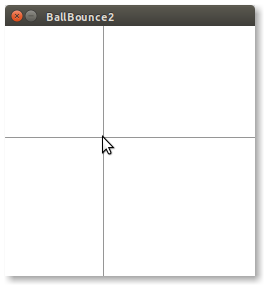
\includegraphics[scale=0.6]{files/BallBounce0}
              \end{center}
        \part Adopt the methods implemented in class as part of our \code{BallBounce} program in order to program a ball that bounces off the newly drawn lines as well as the sides of the window.\\
              \begin{center}
                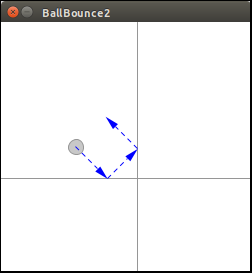
\includegraphics[scale=0.5]{files/BallBounce1} \hspace{2cm} 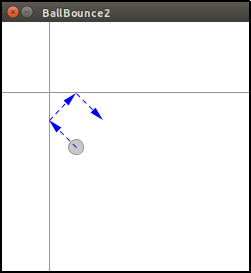
\includegraphics[scale=0.5]{files/BallBounce2}
              \end{center}
        \part Modify your program to allow the ball to pass through the drawn lines when the mouse button is held down. Implement some visual clue that indicates the ball will be allowed to pass.
      \end{parts}
    }
  \end{questions}
\end{document}
